%\section{Approximating solutions of equations}

 \begin{center}
\line(1,0){300} %\line(1,0){250}
\end{center}

\section*{Homework}

\noindent \textbf{Start by doing Practice exercises \#1-4 in the workbook.}

\bigskip

\noindent \textbf{Do you know \ldots}

\begin{itemize} 
\item What a solution to an equation is? 
\item When you approximate a solution of an equation, as opposed to just evaluating? 
\item How to use successive approximation, including organizing your work in a table? 
\item How to get a reasonable first guess from a graph? 
\item What to do if you do not have a reasonable first guess? 
\item How precise your answer should be? 
\item How to find numbers between given numbers, for example between .3 and .4? 
 \item[~] \textbf{If you're not sure, work the rest of exercises and then return to these questions.  Or, ask your instructor or a classmate for help.} 
\end{itemize}

\subsection*{Exercises}

\begin{enumerate} 
\setcounter{enumi}{4}

\item  The population of China in 2011 was approximately 1.343 billion and growing at around .48\% per year.  An equation estimating the population of China is
$$P = 1.343 \ast 1.0048^Y$$ where $P$ is the population of China (measured in billions) and $Y$ is the years since 2011. \hfill \begin{footnotesize} Source:  CIA Factbook \end{footnotesize}
\begin{enumerate}
\item In what year is China's population projected to reach 1.5 billion?
\item In what year is India's population expected to pass China's?  Remember that we discussed India's population in this section.
 \item Explain how we got the equation for China.
 \item Draw graph showing both equations.
\end{enumerate} 

\item A company who makes electronics was doing great business in 1996, but sales quickly slid after 2000.  Their sales $M$ in millions of \$ $Y$ years from 1996 is given by the following equation $$M = 104.4+11.5Y-1.4Y^2$$
\hfill \emph{Story appears in 3.5 Exercises}
\begin{enumerate}
\item What were the company's sales in 1996, 2000, 2005?
\item The company decided to declare bankruptcy when sales fell below \$20 billion.  In what year was that?  Show how to use successive approximations to estimate the answer to the nearest year. 
\item An analyst had suggested that they close down shop earlier, once sales were below \$50 billion.  In what year did sales fall that low? Again, use successive approximation.
\end{enumerate} 

\item Suppose a special kind of window glass is 1 inch thick and lets through only 75\% of the light. If two thicknesses of this glass are used, the product is 2 inches thick and lets in 56.25\% since $$75\% \text{ of } 75\% = (.75)(.75) = .5625 = 56.25\%$$ 
 \hfill \emph{Story also appears in 3.4 and 5.4 Exercises}
\begin{enumerate}
\item If three thickness of this glass is used, explain why the product is 3 inches think and lets in about 42.19\% of the light.
\item If four thickness of this glass is used, how thick will the product be and what percentage (\%) of the light will be let through?
\item Identify and name the variables, including their units, and write an equation relating them.
\item Use successive approximation to figure out what thickness glass should be used to let through less than 10\% of the light. Display your work in a table.
\item Graph the function.
\end{enumerate} 

\item Wind turbines are used to generate electricity.  For a particular wind turbine, the equation $$W = 2.4 S^3$$ can be used to calculate the amount of electricity generated ($W$ watts) for a given wind speed ($S$ mph), over a fixed period of time.

\hfill \emph{Story also appears in 1.1, 1.3, and 3.3 Exercises}
\begin{enumerate}
\item Make a table showing the amount of electricity produced when the wind speed is 10 mph, 25 mph, and 40 mph. 
\item Draw a graph illustrating this equation.
\item Approximate the wind speed that will generate 12,500 watts of electricity. 
\end{enumerate} 

\item After his first beer, Stephen's blood alcohol content (BAC) was already .04 and as he continued to drink, his BAC level rose 45\% per hour.  The equation is $$S = .04 \ast 1.45^H$$ where $S$ is Stephen's BAC and $H$ is the time, measured in hours.

\hfill \emph{Story also appears in 1.1 \#4 and 3.4 \#1} 
\begin{enumerate}
\item Make a table showing Stephen's BAC at the start of the problem and each of the next four hours.
\item Draw a graph showing how Stephen's BAC changed over time.
\item At a BAC of .10 it is illegal for Stephen to drive.  Approximately when does that happen?
\end{enumerate}  

\item Urban community gardens are catching on.  What was once an abandoned lot down the block is now a thriving 10'$\times$25' vegetable and berry garden for the neighborhood. One neighbor volunteered to donate gravel to make a path around the garden.  The path will be 3 inches deep and the same width all around.   The amount of gravel they need ($G$ cubic feet) is given by the equation  $$G = W^2 + 17.5W$$
where $W$ is the width of the path in feet.  
\begin{center}
\scalebox {.4} {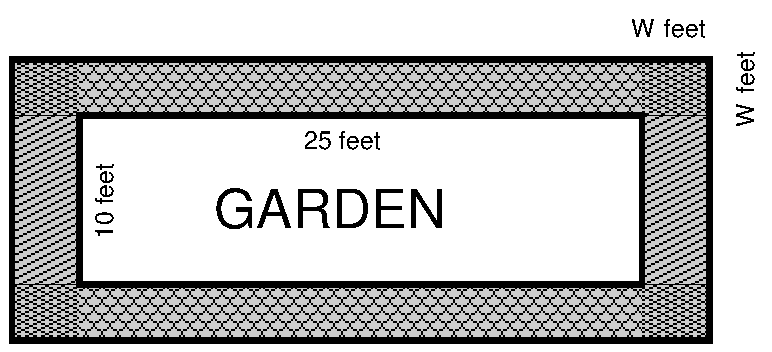
\includegraphics{GravelPath.pdf}}
\end{center}
 \hfill \emph{Story also appears in 2.3 Exercises and 3.5 \#4}
\begin{enumerate}
\item  If the neighbor donates 60 cubic feet of gravel, how wide a path can they build?  Report your answer to two decimal places. 
\item Convert your answer to feet and inches.  Do you think that's a wide enough path? 
\end{enumerate}

\end{enumerate}
